\documentclass{article}

% if you need to pass options to natbib, use, e.g.:
% \PassOptionsToPackage{numbers, compress}{natbib}
% before loading nips_2018

% ready for submission
% \usepackage{nips_2018}

% to compile a preprint version, e.g., for submission to arXiv, add
% add the [preprint] option:
\usepackage[final]{nips_2018}

% to compile a camera-ready version, add the [final] option, e.g.:
% \usepackage[final]{nips_2018}

% to avoid loading the natbib package, add option nonatbib:
% \usepackage[nonatbib]{nips_2018}

\usepackage[utf8]{inputenc} % allow utf-8 input
\usepackage[T1]{fontenc}    % use 8-bit T1 fonts
\usepackage{hyperref}       % hyperlinks
\usepackage{url}            % simple URL typesetting
\usepackage{booktabs}       % professional-quality tables
\usepackage{amsfonts}       % blackboard math symbols
\usepackage{amsmath}
\usepackage{nicefrac}       % compact symbols for 1/2, etc.
\usepackage{microtype}      % microtypography
\usepackage{subfig}
\usepackage[pdftex]{graphicx}
\graphicspath{ {img/} }

\newcommand{\norm}[1]{\left\lVert#1\right\rVert}

\title{Recurrent Neural Networks for Time Series Prediction}

% The \author macro works with any number of authors. There are two
% commands used to separate the names and addresses of multiple
% authors: \And and \AND.
%
% Using \And between authors leaves it to LaTeX to determine where to
% break the lines. Using \AND forces a line break at that point. So,
% if LaTeX puts 3 of 4 authors names on the first line, and the last
% on the second line, try using \AND instead of \And before the third
% author name.

\author{
  Davide Spallaccini\thanks{\texttt{spallaccini.1642557@studenti.uniroma1.it}}
\\
  Department of Computer, Control \\ and Management Engineering\\
  Sapienza University of Rome\\
  Rome, Italy \\
  \And
  Beatrice Bevilacqua\thanks{\texttt{bevilacqua.1645689@studenti.uniroma1.it}}
\\
  Department of Computer, Control \\ and Management Engineering\\
  Sapienza University of Rome\\
  Rome, Italy \\
   \\
  %% examples of more authors
  \And
  Anxhelo Xhebraj\thanks{\texttt{xhebraj.1643777@studenti.uniroma1.it}} \\
  Department of Computer, Control \\ and Management Engineering\\
  Sapienza University of Rome\\
  Rome, Italy
  %% Affiliation \\
  %% Address \\
  %% \texttt{email} \\
  %% \AND
  %% Coauthor \\
  %% Affiliation \\
  %% Address \\
  %% \texttt{email} \\
  %% \And
  %% Coauthor \\
  %% Affiliation \\
  %% Address \\
  %% \texttt{email} \\
  %% \And
  %% Coauthor \\
  %% Affiliation \\
  %% Address \\
  %% \texttt{email} \\
}

\begin{document}
% \nipsfinalcopy is no longer used

\maketitle

\begin{abstract}

Recently recurrent neural networks due to their ability to capture
time-dependent
features have been applied to time series forecasting showing important
improvements with respect to previous methods. Simple RNN architectures though
suffer from vanishing/exploding gradient problems and cannot discriminate
exogenous series in case these are given as input. In this work we analyse a
solution based on LSTM networks and a multiple attentions mechanism and compare
this to simpler models including a multistep-ahead encoder-decoder architecture
to show the effectiveness of the method proposed by [1].

\end{abstract}

\section{Introduction and Related Work}
\label{sec:intro}

Nonlinear autoregressive exogenous models (NARX) aim to predict the current
value $y_T$ of a time series $y$ based on its
collected knowledge coming from the past $T -1$ values ($T$ also denoted as
window size) of
the time series ($y_{1}, y_{2}, ..., y_{T-1}$) and the current and past $T$
values of $n$
exogenous time series ($\mathbf{x}_{1}, \mathbf{x}_{2}, ..., \mathbf{x}_{T}$)
, $\mathbf{x}_t \in \mathbb{R}^n$ where $\mathbf{x}_t = (x_t^1, x_t^2, ...,
x_t^n)^\top$
are the values of each driving series at timestep $t$ and $\mathbf{x}^k =
(x_1^k, x_2^k, ..., x_T^k)$ are the values of the $k$-th time series in a given
window. Exogenous time series
are data that may be correlated to the series under consideration, so they are
also called \textit{driving series}. A good NARX algorithm should be able to
choose which of the series are to be
considered driving when predicting the current value of the target series.
At the same time, a good algorithm should be able to capture long-term temporal
dependencies.

In this work we analyse a deep-learning-based model that tries to tackle
these two issues through the usage of
recurrent neural networks and a carefully combined system of attention
mechanisms. We perform an ablation study that wasn't directly reported in the
authors' paper to validate the effectiveness of the approach proposed and
compare the result with other possible approaches to the same problem using
again recurrent networks.
Classic statistical models, though effective for some real word applications,
do not perform very well since they cannot
model nonlinear relationships and do not differentiate between driving terms, or
they model nonlinear relationships
but with a predefined nonlinear relationship which is not necessarily the true
underlying one.

\section{Dataset}
\label{sec:retrieval}

We used the same datasets as the authors' in order to try to compare our results
with the ones reported.

The first dataset is SML 2010; its task is to predict the temperature of indoor
environments. The data is collected from sensors of a system mounted in a
domestic house for a total time of 40 days. The data is sampled every minute
and
was smoothed with 15 minutes mean. The target series we select is the room
temperature and we collect 17 driving series by filtering out series which
are constant. We use $80$ percent of the dataset for training and we
split evenly the remaining between validation and test.

The second dataset is the NASDAQ 100 Stock dataset which is characterised by a
larger number of driving series and stronger variations. This dataset is
made public by the same
authors of the original paper and is a collection of prices of 81 major
corporations under NASDAQ 100 used as driving time series. The target series
used is the value of the NASDAQ 100 index. The frequency of the data is
minute-by-minute and covers 105 days from July 26, 2016 to December 22, 2016.
We use $80$ percent of the dataset for training, and the remaining is split
into
validation and test.

Both datasets are transformed into overlapping windows of a given size
$T$ (with the last value of the target series being the one we aim to predict),
with stride 1.

\begin{figure}[h]
\centering
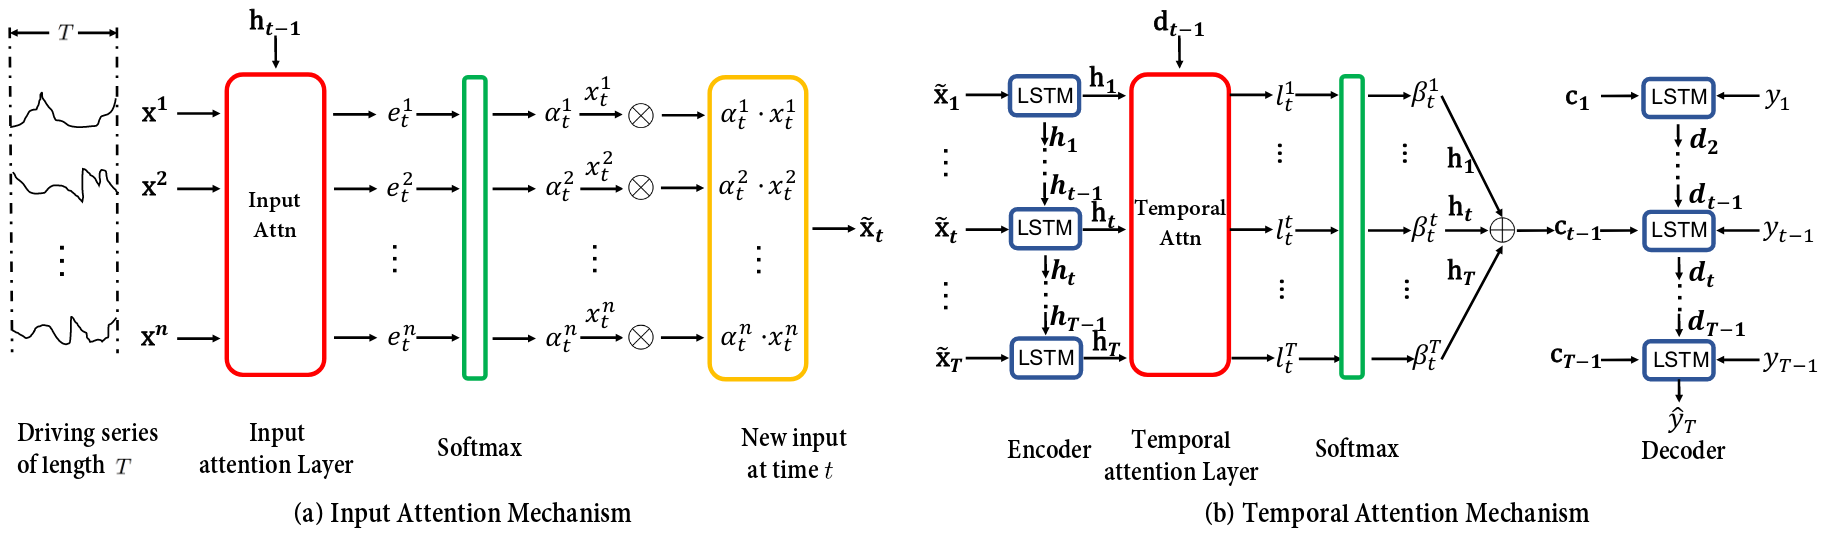
\includegraphics[width=\linewidth]{da-rnn.png} \\
\caption{DA-RNN model}

\label{fig:da-rnn}
\end{figure}


\section{Dual-stage attention model}
\label{sec:da-rnn}

The proposed model of the reference paper, which is illustrated in Figure
\ref{fig:da-rnn},
introduces two attention mechanisms in a LSTM-based encoder and decoder
architecture.
The first attention, \textit{Input Attention}, is trained to independently
weight
the driving series at each timestep producing
\begin{align*}
(\tilde{\mathbf{x}}_1, \tilde{\mathbf{x}}_2, ..., \tilde{\mathbf{x}}_T) =
A_{in}((\mathbf{x}_1, \mathbf{x}_2, ..., \mathbf{x}_T)) =
(\boldsymbol{\alpha}_1 \odot \mathbf{x}_1, \boldsymbol{\alpha}_2 \odot
\mathbf{x}_2, ..., \boldsymbol{\alpha}_T \odot \mathbf{x}_T)
\end{align*}
with $\boldsymbol{\alpha}_i \in \mathbb{R}^n$ and
$\norm{\boldsymbol{\alpha}_i}_1 = 1$.
This helps in highlighting which series are useful for the prediction of
the target series.

The weighted driving series are than passed to a one layer LSTM encoder of
which hidden states (cell state and hidden state) are used in the Input
Attention
mechanism.

For each timestep the encoder maps the "attentioned" input
$\tilde{\mathbf{x}}_t$ to a vector
$\mathbf{h}_t \in \mathbb{R}^m$ which is the hidden state of
the LSTM at timestep $t$. The operations involved in this mapping are the ones
that take place in the update of a LSTM cell and can be summarised as follows:


\begin{equation} \label{eq:lstm}
\begin{split}
\mathbf{f}_t &= \sigma (\mathbf{W}_f[\mathbf{h}_{t-1};\tilde{\mathbf{x}}_t] +
\mathbf{b}_f) \\
\mathbf{i}_t &= \sigma (\mathbf{W}_i[\mathbf{h}_{t-1};\tilde{\mathbf{x}}_t] +
\mathbf{b}_i) \\
\mathbf{o}_t &= \sigma (\mathbf{W}_o[\mathbf{h}_{t-1};\tilde{\mathbf{x}}_t] +
\mathbf{b}_o) \\
\mathbf{s}_t &= \mathbf{f}_t \odot \mathbf{s}_t + \mathbf{i}_t
				\odot
\text{tanh}(\mathbf{W}_s[\mathbf{h}_{t-1};\tilde{\mathbf{x}}_t] + \mathbf{b}_s)
\\
\mathbf{h}_t &= \mathbf{o}_t \odot \text{tanh}(\mathbf{s}_t)
\end{split}
\end{equation}

Where $[\mathbf{h}_{t-1};\tilde{\mathbf{x}}_t] \in \mathbb{R}^{m + n}$ is a
concatenation of the hidden state of the previous
timestep and the input of the current timestep;
$\mathbf{W}_f,\mathbf{W}_i,\mathbf{W}_o,\mathbf{W}_s
\in \mathbb{R}^{m \times(m+n)}$, and $\mathbf{b}_f, \mathbf{b}_i,
\mathbf{b}_o,\mathbf{b}_s \in \mathbb{R}^m$ are
parameters to learn; $\sigma$ and $\odot$ are a logistic sigmoid function and
an element-wise multiplication,
respectively.

The second attention mechanism introduced, \textit{Temporal Attention},
adaptively
selects relevant encoder hidden states across the timesteps of the window
producing
\begin{align*}
(\mathbf{c}_1, \mathbf{c}_2, ..., \mathbf{c}_T) = A_{temp}((\mathbf{h}_1,
\mathbf{h}_2, ..., \mathbf{h}_T)) =
\left(\sum_{i=1}^T \beta_1^i \mathbf{h}_i, \sum_{i=1}^T \beta_2^i\mathbf{h}_i,
..., \sum_{i=1}^T \beta_T^i\mathbf{h}_i \right)
\end{align*}
where $\beta^i_t$ represents the importance of the $i$-th encoder
hidden state for the prediction.

The $t$-th "attentioned" encoder hidden state $\mathbf{c}_t$ is then
concatenated with
$y_t$, given in input to a dense layer of which output is then fed in input
to the decoder. When $t = T$ instead, the "attentioned" encoder hidden state is
concatenated to the hidden state of the decoder and passed to two dense layers
to obtain the predicted value.


For the Input Attention, the following operations are taken to
obtain the weights $\alpha_t^k$

\begin{align*}
e_t^k &= \mathbf{v}_e^\top\text{tanh}(
		 \mathbf{W_e}[\mathbf{h}_{t-1};\mathbf{s}_{t-1}]
+\mathbf{U_e}\mathbf{x}^k), & 1 \le k \le n \\
\alpha_t^k &= \frac{\text{exp}(e_t^k)}{\sum_{i=1}^n \text{exp}(e_t^i)},
\end{align*}

where $\mathbf{h}_{t-1}, \mathbf{s}_{t-1}$ are the hidden and cell states
of the encoder, $\mathbf{x}^k$ is one driving series,
$\mathbf{v}_e \in \mathbb{R}^T, \mathbf{W}_e \in \mathbb{R}^{T\times 2m}$ and
$\mathbf{U}_e \in \mathbb{R}^{T\times T}$ (with $m$ the hidden size of the
encoder)
are learnable parameters.

For the Temporal Attention, the following operations are taken to
obtain the weights $\beta_t^i$

\begin{align*}
l_t^i &= \mathbf{v}_d^\top\text{tanh}(
		 \mathbf{W_d}[\mathbf{d}_{t-1};\mathbf{s}'_{t-1}]
+\mathbf{U_d}\mathbf{h}_i), & 1 \le i \le T \\
\beta_t^i &= \frac{\text{exp}(l_t^i)}{\sum_{i=1}^n \text{exp}(e_t^i)},
\end{align*}

where $\mathbf{d}_{t-1}, \mathbf{s}'_{t-1} \in \mathbb{R}^p$ are the hidden and
cell states
of the decoder, $\mathbf{h}_i$ is the $i$-th hidden state of the encoder,
$\mathbf{v}_d \in \mathbb{R}^m, \mathbf{W}_d \in \mathbb{R}^{m \times 2p}$ and
$\mathbf{U}_d \in \mathbb{R}^{m\times m}$ (with $p$ the hidden size of the
decoder)
are learnable parameters.

\subsection{Implementation details}

We used Tensorflow $1.12$ as the target framework to implement the model just
described. The reason behind this choice is that we
could easily translate the equations of the model directly into the code and
define each step of the model pragmatically.


For the encoder network we used the \texttt{LSTMCell} class from
\texttt{tensorflow.python.ops.rnn\_cell\_impl}.
We initially instantiated a zero state for the cell and the hidden states. Then
for each timestep we defined the Tensorflow computational graph nodes, in
particular
the nodes for the Input Attention implementation and the \texttt{LSTMCell},
which takes
as input the hidden state of the previous timestep and the
output of the Input Attention. During this process we collect the output hidden
states of the cell for the various timesteps, that is finally reshaped
to be the input of the Temporal Attention.

For the decoder network implementation we instantiated a zero state for the
cell and
the hidden state and we defined the nodes for the Temporal attention. The
target series value at time $t$ is concatenated with the output of the temporal
attention
at time $t$ and passed to a dense layer. The newly computed vector is used for
the
update of the decoder hidden state in the \texttt{LSTMCell}. For $y_T$, which
is what we aim to predict, the "attentioned" encoder hidden state at time $T$
is concatenated to the last hidden state of the decoder and fed to two dense
layers.

To make the experimentation modular we defined a data class that loads all
the parameters and file paths from JSON configuration files.

Initially, in order to ensure the correctness of the formulas being implemented
we used the Eager Execution model offered by Tensorflow which allows to easily
debug and quickly iterate over the core of the model.

We used Tensorboard to graphically visualize the value of the loss across
the training steps and the values of the evaluation metrics on the validation
set
at every epoch of training.

Finally we exploited the checkpointing facilities
offered by the framework to save two main set of values: the data needed to
restart the training on a successive run of the training and the weights of the
model that achieved the best performance in all the evaluation sessions. The
final
tests indeed are done by loading the weights of the best model even if the
training ran for longer or later incurred in overfitting.



\newpage

\begin{figure}[h]
  \centering
  \subfloat[SML 2010 validation set]{{
    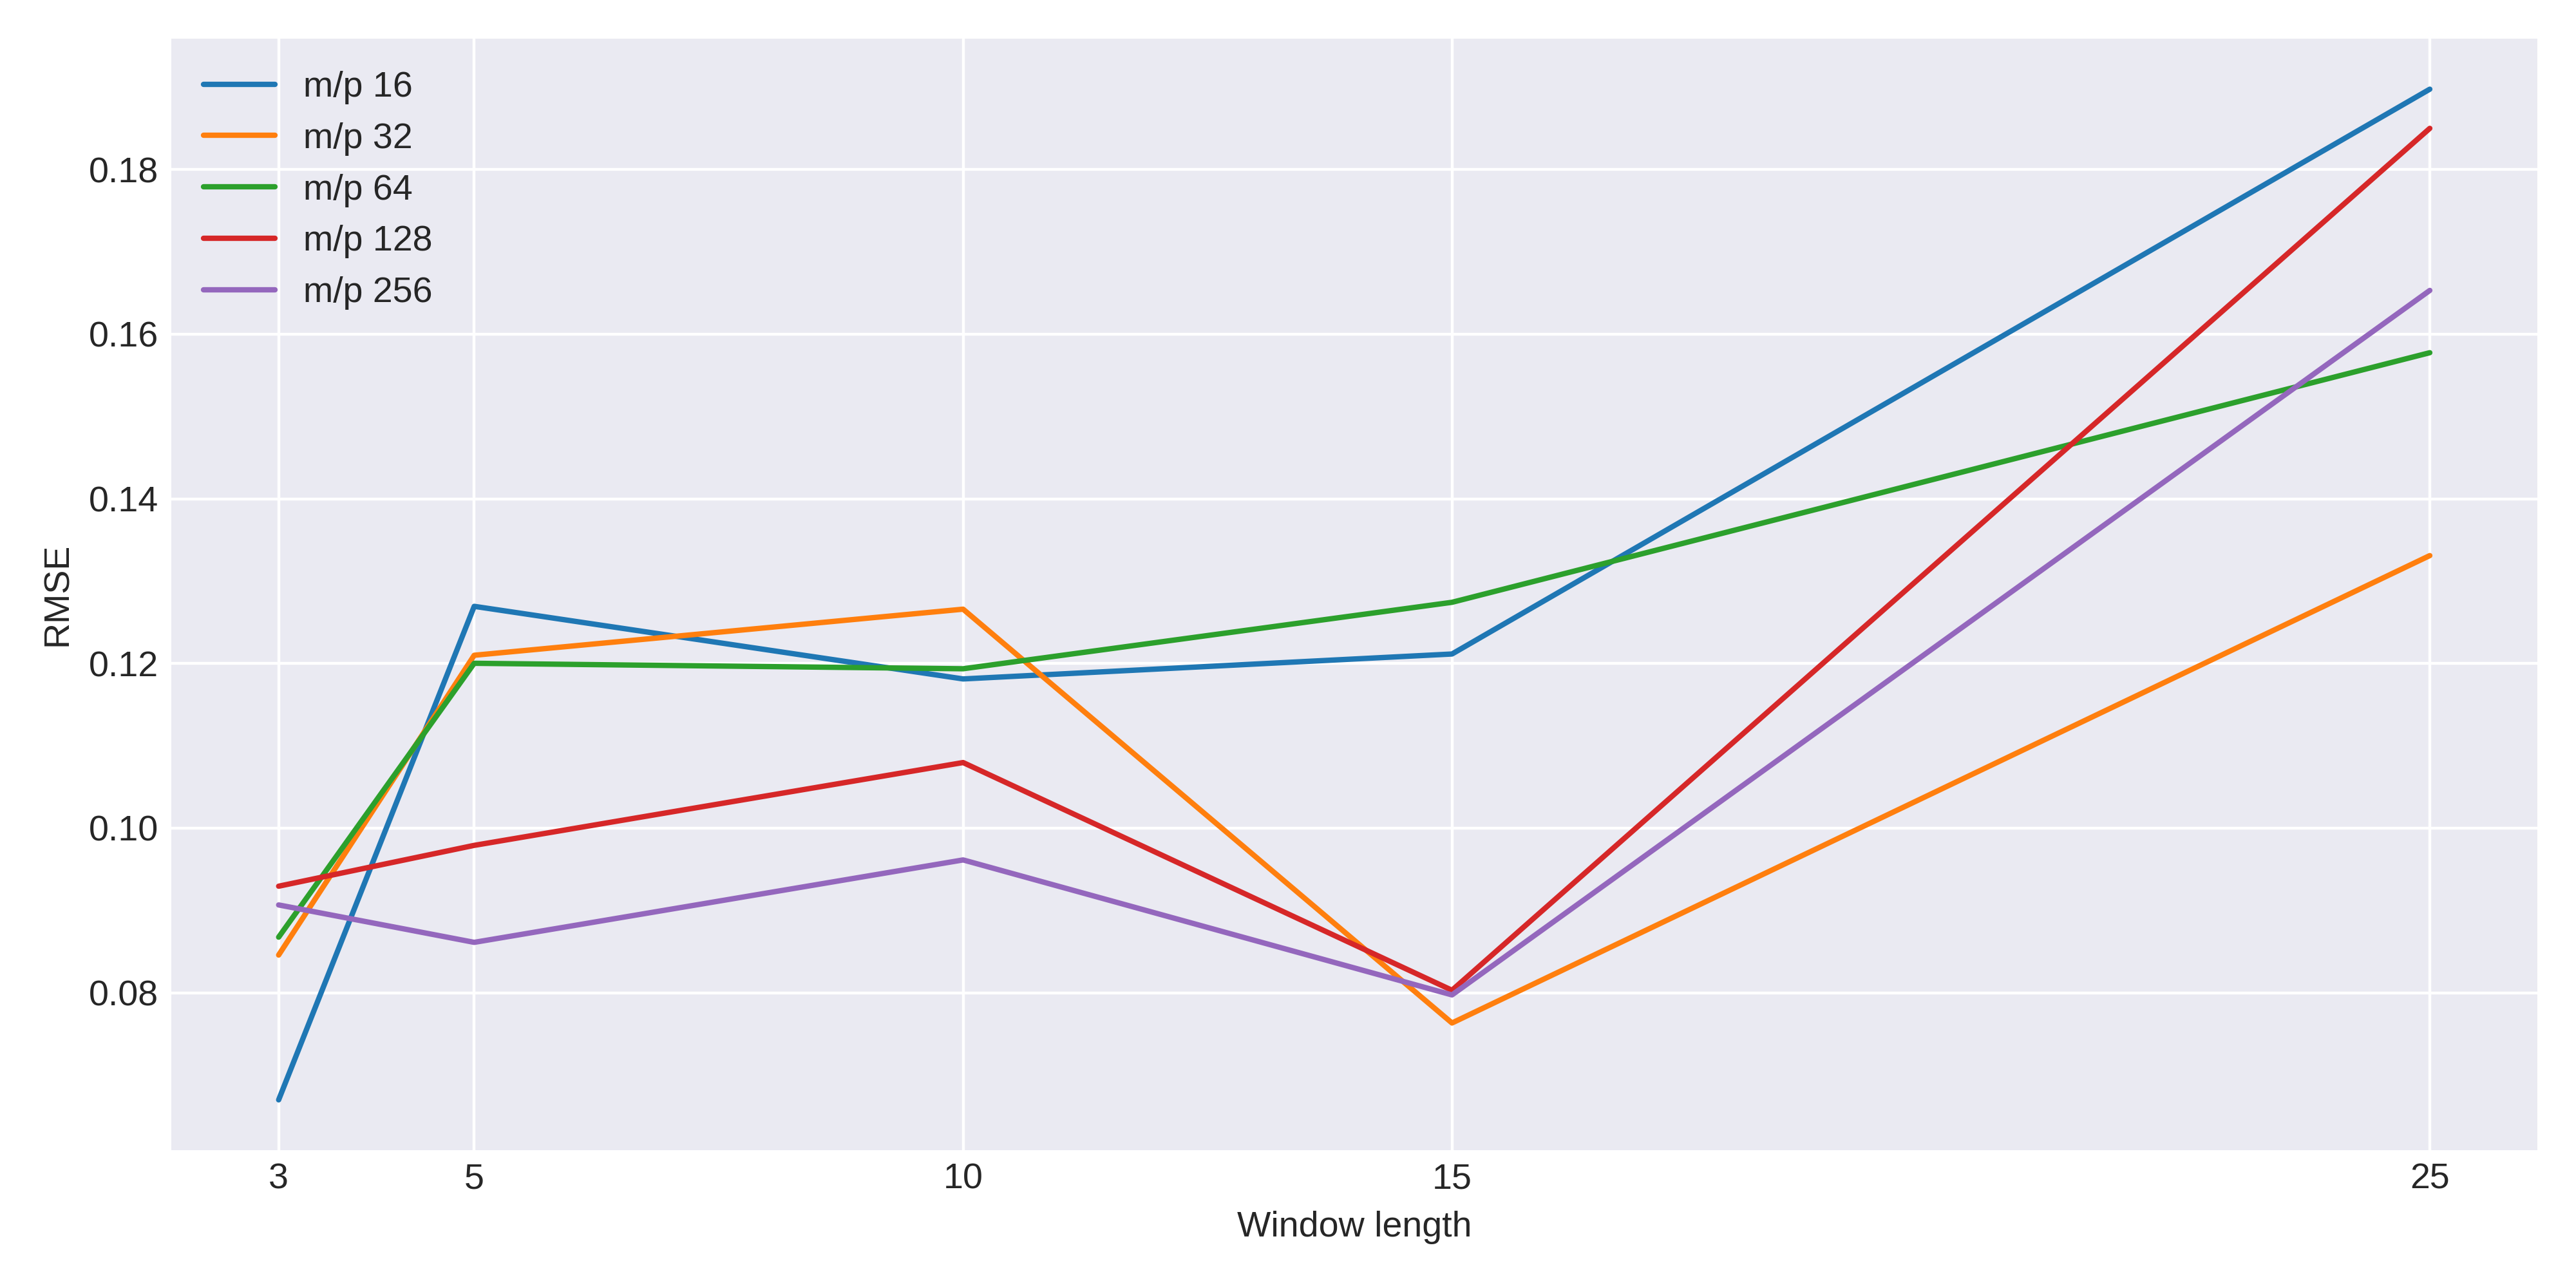
\includegraphics[width=0.6\linewidth]{hype-sml.png}
  }} \\
  \subfloat[NASDAQ 100 validation set]{{
    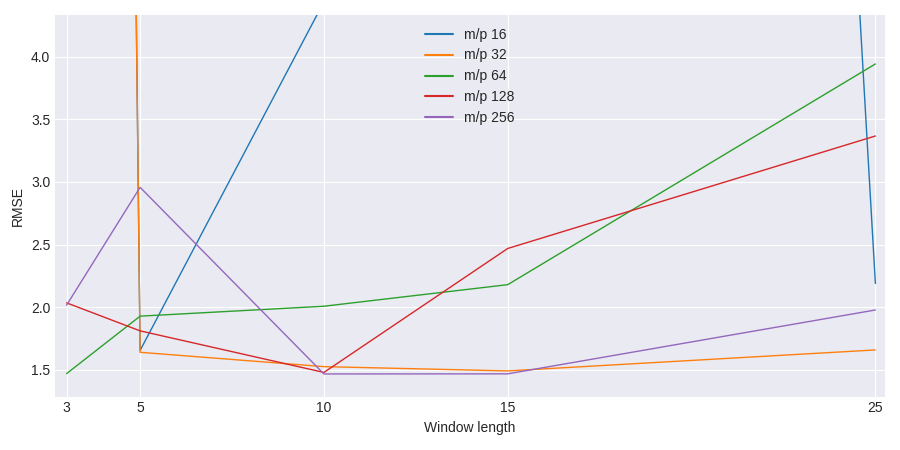
\includegraphics[width=0.6\linewidth]{hype-nasdaq.png}
  }}
  \caption{RMSE score across the dataset for different
   window lengths $T$ and encoder/decoder hidden state size,
   $m$ and $p$ respectively}
  \label{fig:hype}
\end{figure}

\subsection{Hyper parameter tuning}

We validated our implementation using the same set of metrics as the original
authors (RMSE, MAE, MAPE) and we performed some hyper-parameter tuning running
the training with
different configuration files.

All the models were trained for 150 epochs using
two Adam optimisers one for the encoder and one for the decoder, which sped up
the training. We used a starting learning rate of 0.001 and exponential decay
with
objective function the Mean Squared Error. We applied clipping of the gradients
to prevent exploding gradients messing up the parameters during training.
The models trained on the SML 2010 dataset were trained with batch size 32 while
the ones trained on NASDAQ 100 with batch size 128. In both cases a grid search
is performed over $T \in \{3, 5, 10, 15, 25\}$ and $m = p \in \{16, 32, 64,
128, 256\}$.
The model with the best performance on the validation set is then used for
further analysis.
In Figure \ref{fig:hype} the RMSE scores as the parameters vary are shown. The
other scores (MAE, MAPE) follow a similar trend. As can be noticed, in general
better
scores are achieved for small window size and as it grows a drop in performance
arises
which is typical of encoder decoder networks [2].

For SML 2010 dataset, given the simplicity of the series to predict, the RMSE
is small even for
small values of the window length. However, since a small window length cannot
capture
long-term dependencies and will also weaken the usefulness of the Temporal
Attention,
we decided to take for test $T = 15$ and $m=p=32$.

For NASDAQ 100 dataset, $T=3$ and $m=p=16$ or $m=p=32$ have high RMSE, since a
small window
size combined with small hidden state sizes does not result effective enough
for the
prediction. For evaluation we take the ones that achieves the best performance,
$T=15$ and $m=p=256$.

After we have obtained a good hyper-parameters setting for the various models
we
compare their performance on our reference datasets.
In Table \ref{results} we show the scores achieved. As can be seen, the results
slightly differ
from the ones of the authors which can be either because of the difference in
the number of epochs
or because of a data normalisation which we did not perform.
\begin{center}
\begin{table}
\begin{tabular}{r|c|c|c|c|c|c|c|c|c|}
\multicolumn{1}{r}{}
  & \multicolumn{3}{c}{\textbf{Train}}
  & \multicolumn{3}{c}{\textbf{Validation}}
  & \multicolumn{3}{c}{\textbf{Test}} \\
  \cline{2-10}
  & \multicolumn{1}{c}{RMSE}
  & \multicolumn{1}{c}{MAE}
  & \multicolumn{1}{c|}{MAPE}
  & \multicolumn{1}{c}{RMSE}
  & \multicolumn{1}{c}{MAE}
  & \multicolumn{1}{c|}{MAPE}
  & \multicolumn{1}{c}{RMSE}
  & \multicolumn{1}{c}{MAE}
  & \multicolumn{1}{c|}{MAPE}\\
\cline{2-10}
NASDAQ100 & 1.7095 & 0.9537 & 0.01991 & 1.4689 & 0.9550 & 0.0198 & 1.5810 &
1.0477 & 0.0212 \\
\cline{2-10}
SML2010 & 0.0644 & 0.0434 & 0.2279 & 0.0763 & 0.0601 & 0.2561 & 0.0863 & 0.0666
& 0.3248 \\
\cline{2-10}
\end{tabular}
\vspace{1em}
\caption{Results over SML2010 and NASDAQ100}
\label{results}
\end{table}
\end{center}

\begin{figure}
  \centering
  \subfloat[SML 2010]{{
    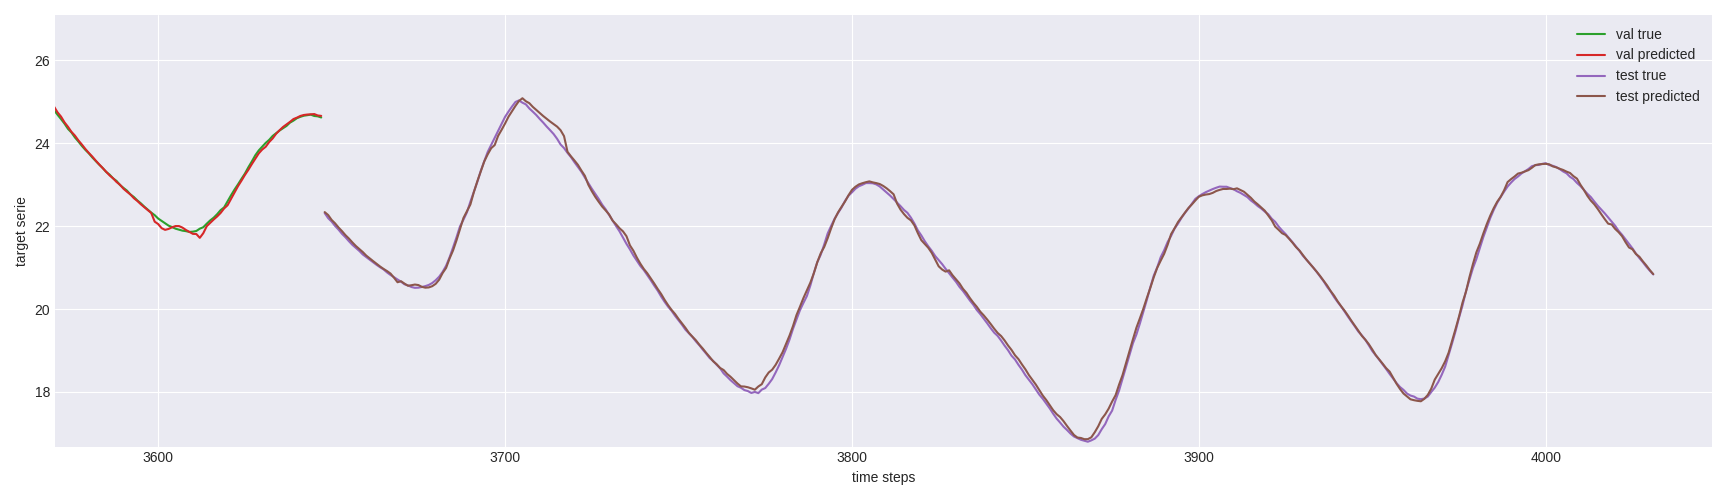
\includegraphics[width=\linewidth]{smlres.png}
  }} \\
  \subfloat[NASDAQ 100]{{
    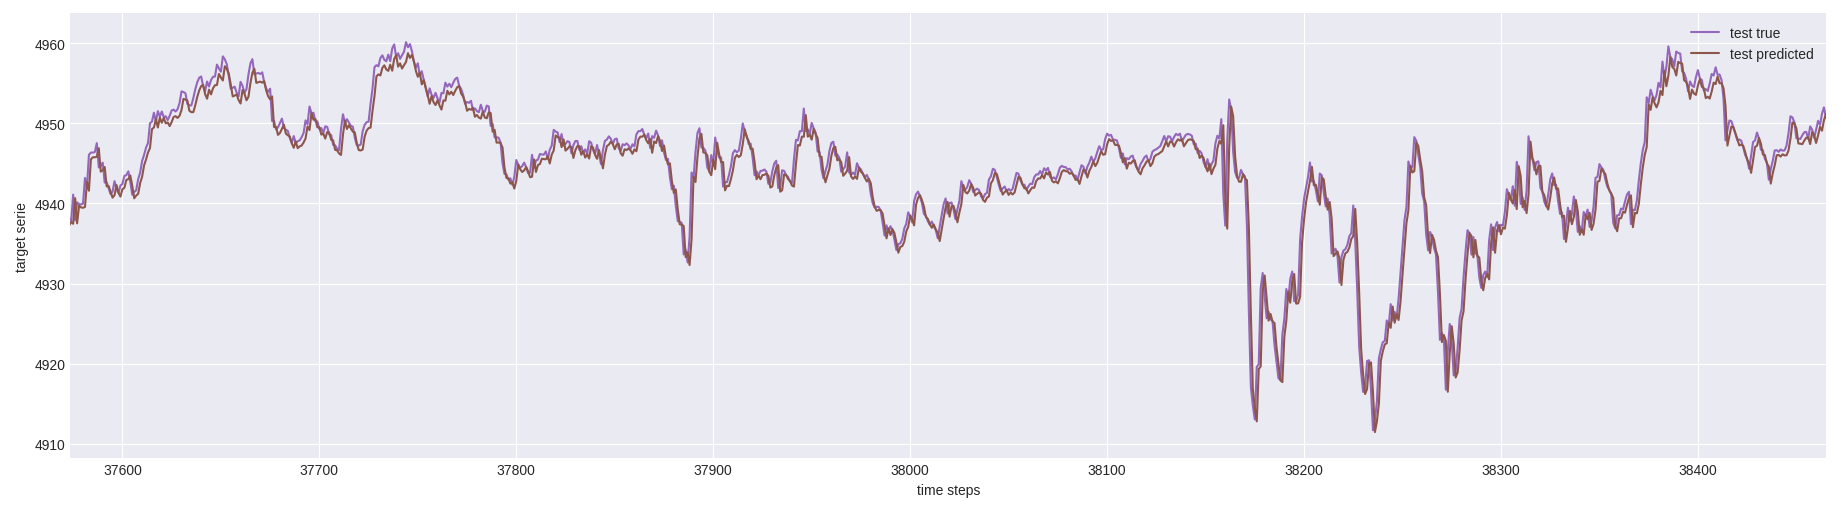
\includegraphics[width=\linewidth]{nasdaqres.png}
  }}
  \caption{Predicted time series and true time series plotted for portions of
the time steps}
  \label{fig:res}
\end{figure}

The results of the predictions are displayed in Figure \ref{fig:res}. As can be
noticed,
the model produces a prediction close to the last seen value of the target
series, with
some small variations.

\subsection{Ablation Study}

\begin{figure}[ht]
  \centering
  \subfloat[SML 2010 test set]{{
    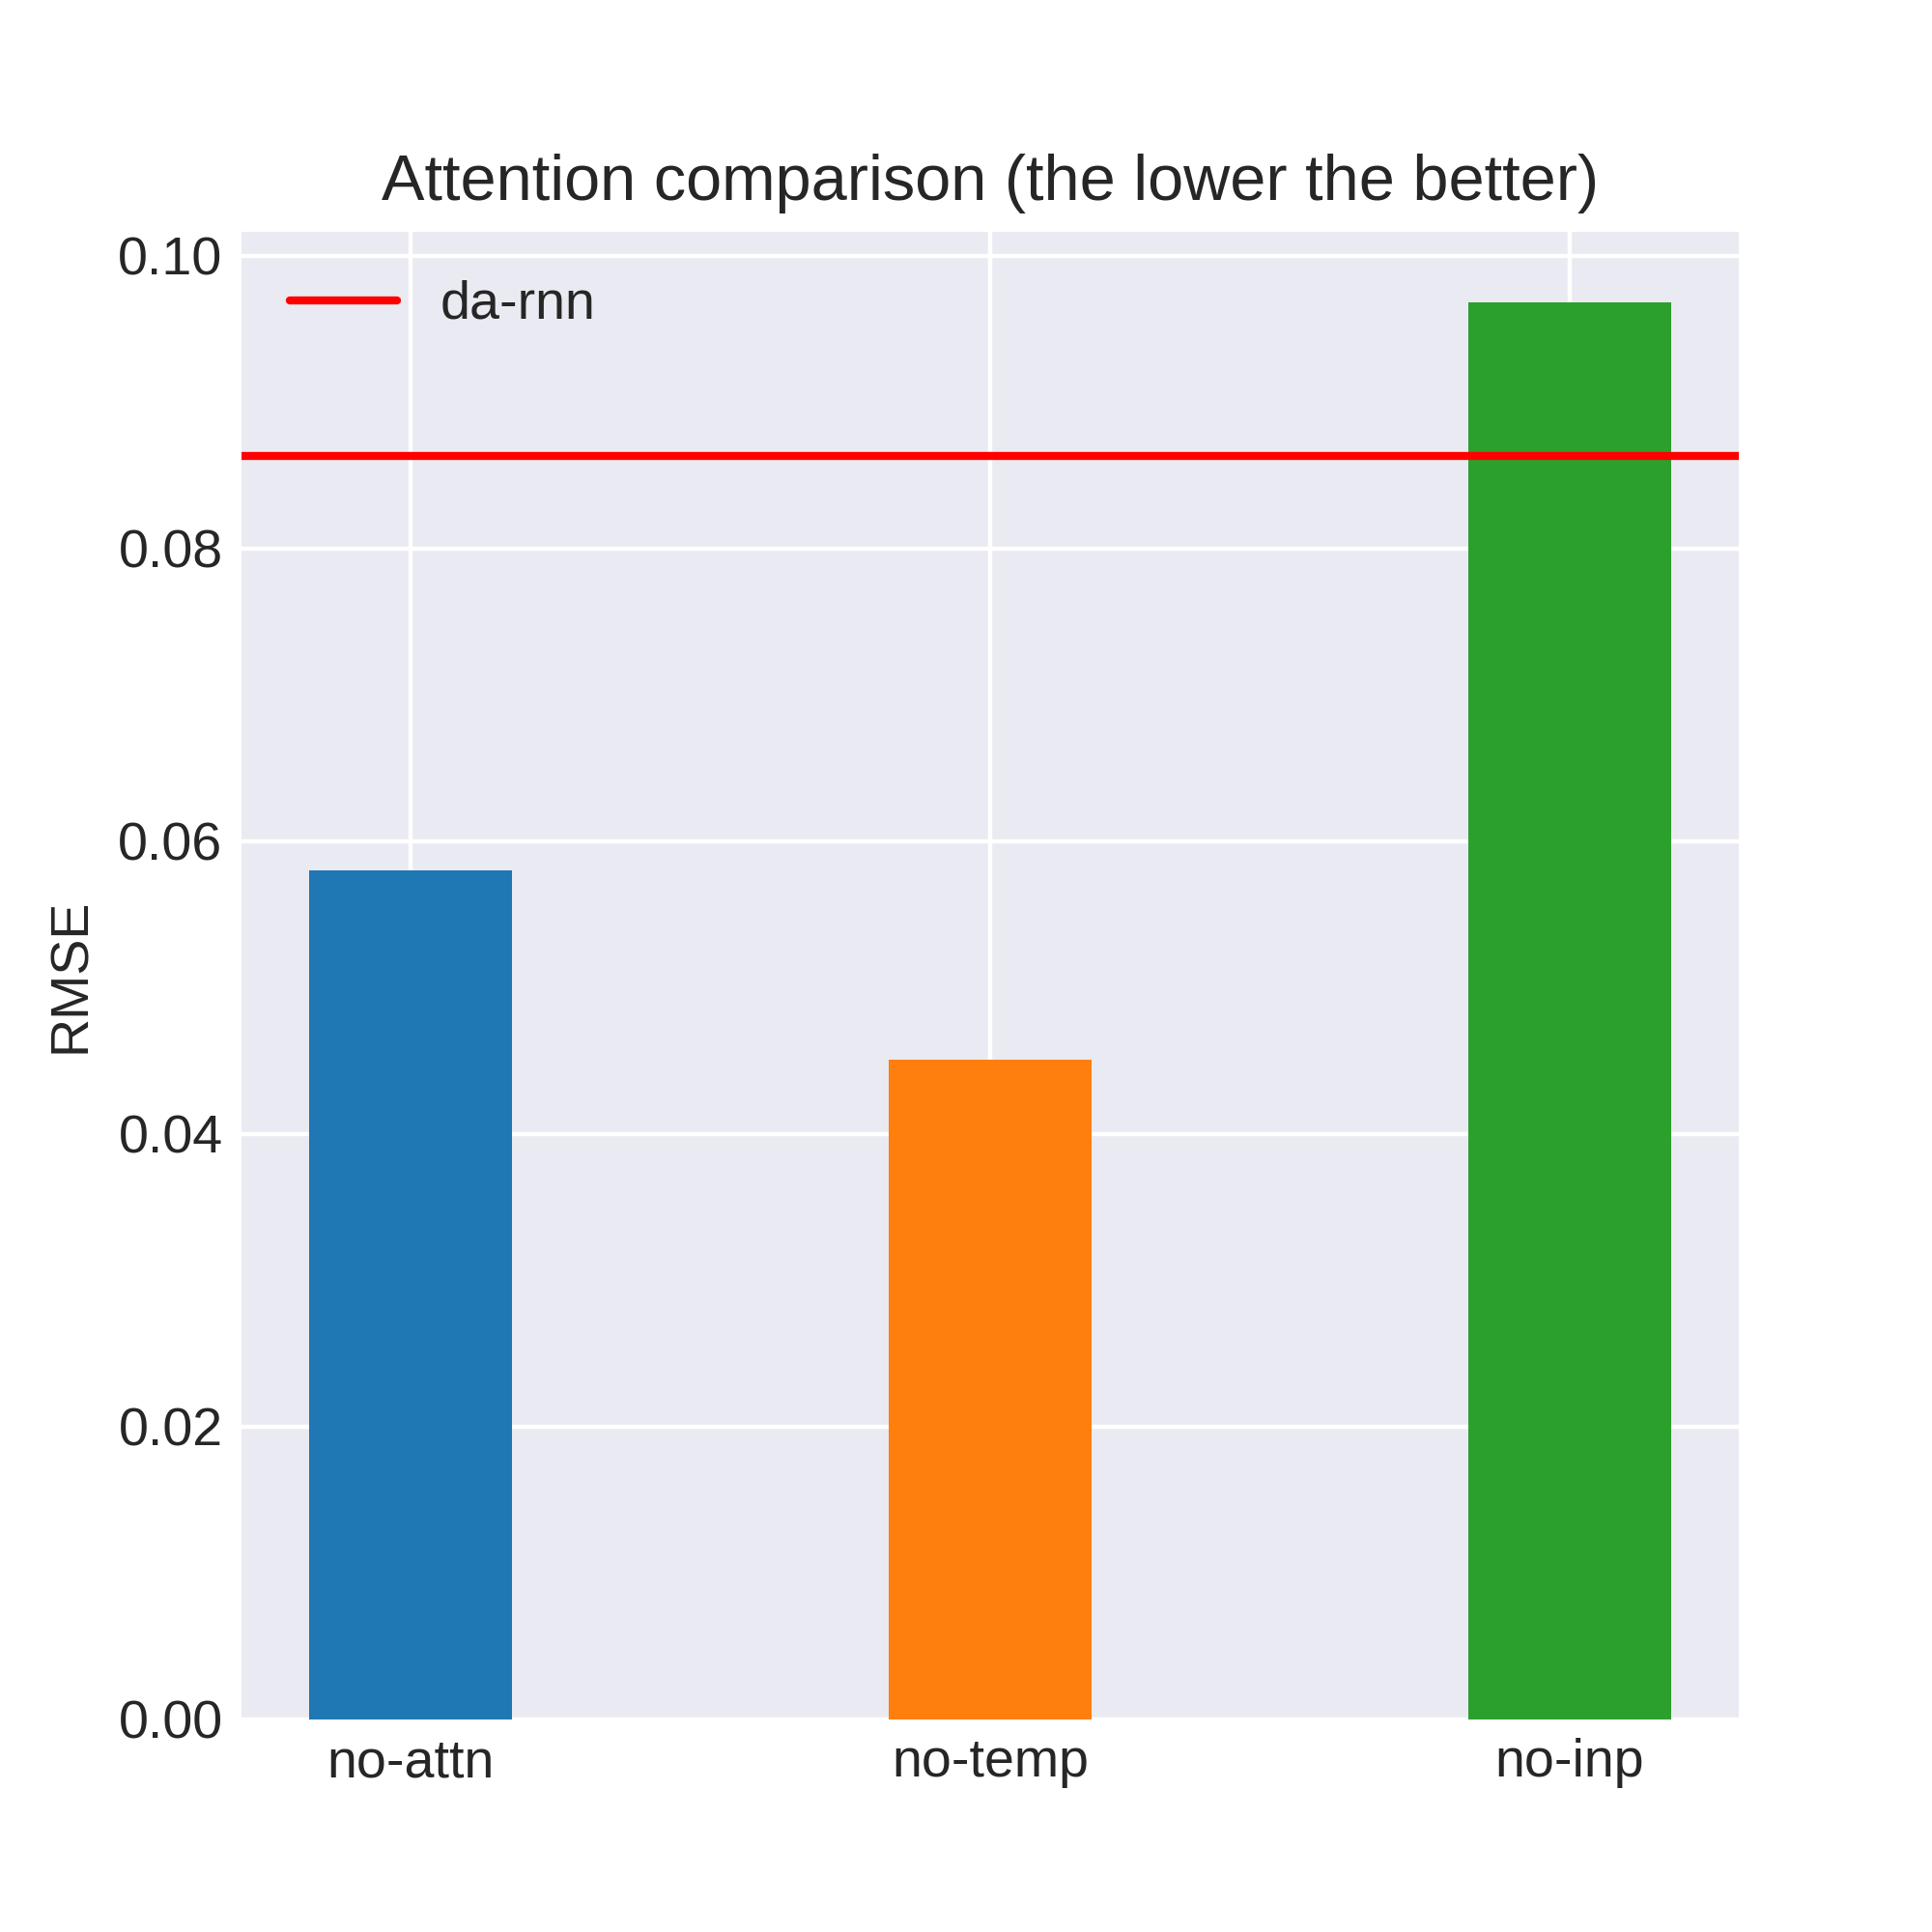
\includegraphics[width=0.4\linewidth]{ablation-sml.png}
    \label{fig:ablation-sml}
  }}
  \subfloat[NASDAQ 100 test set]{{
    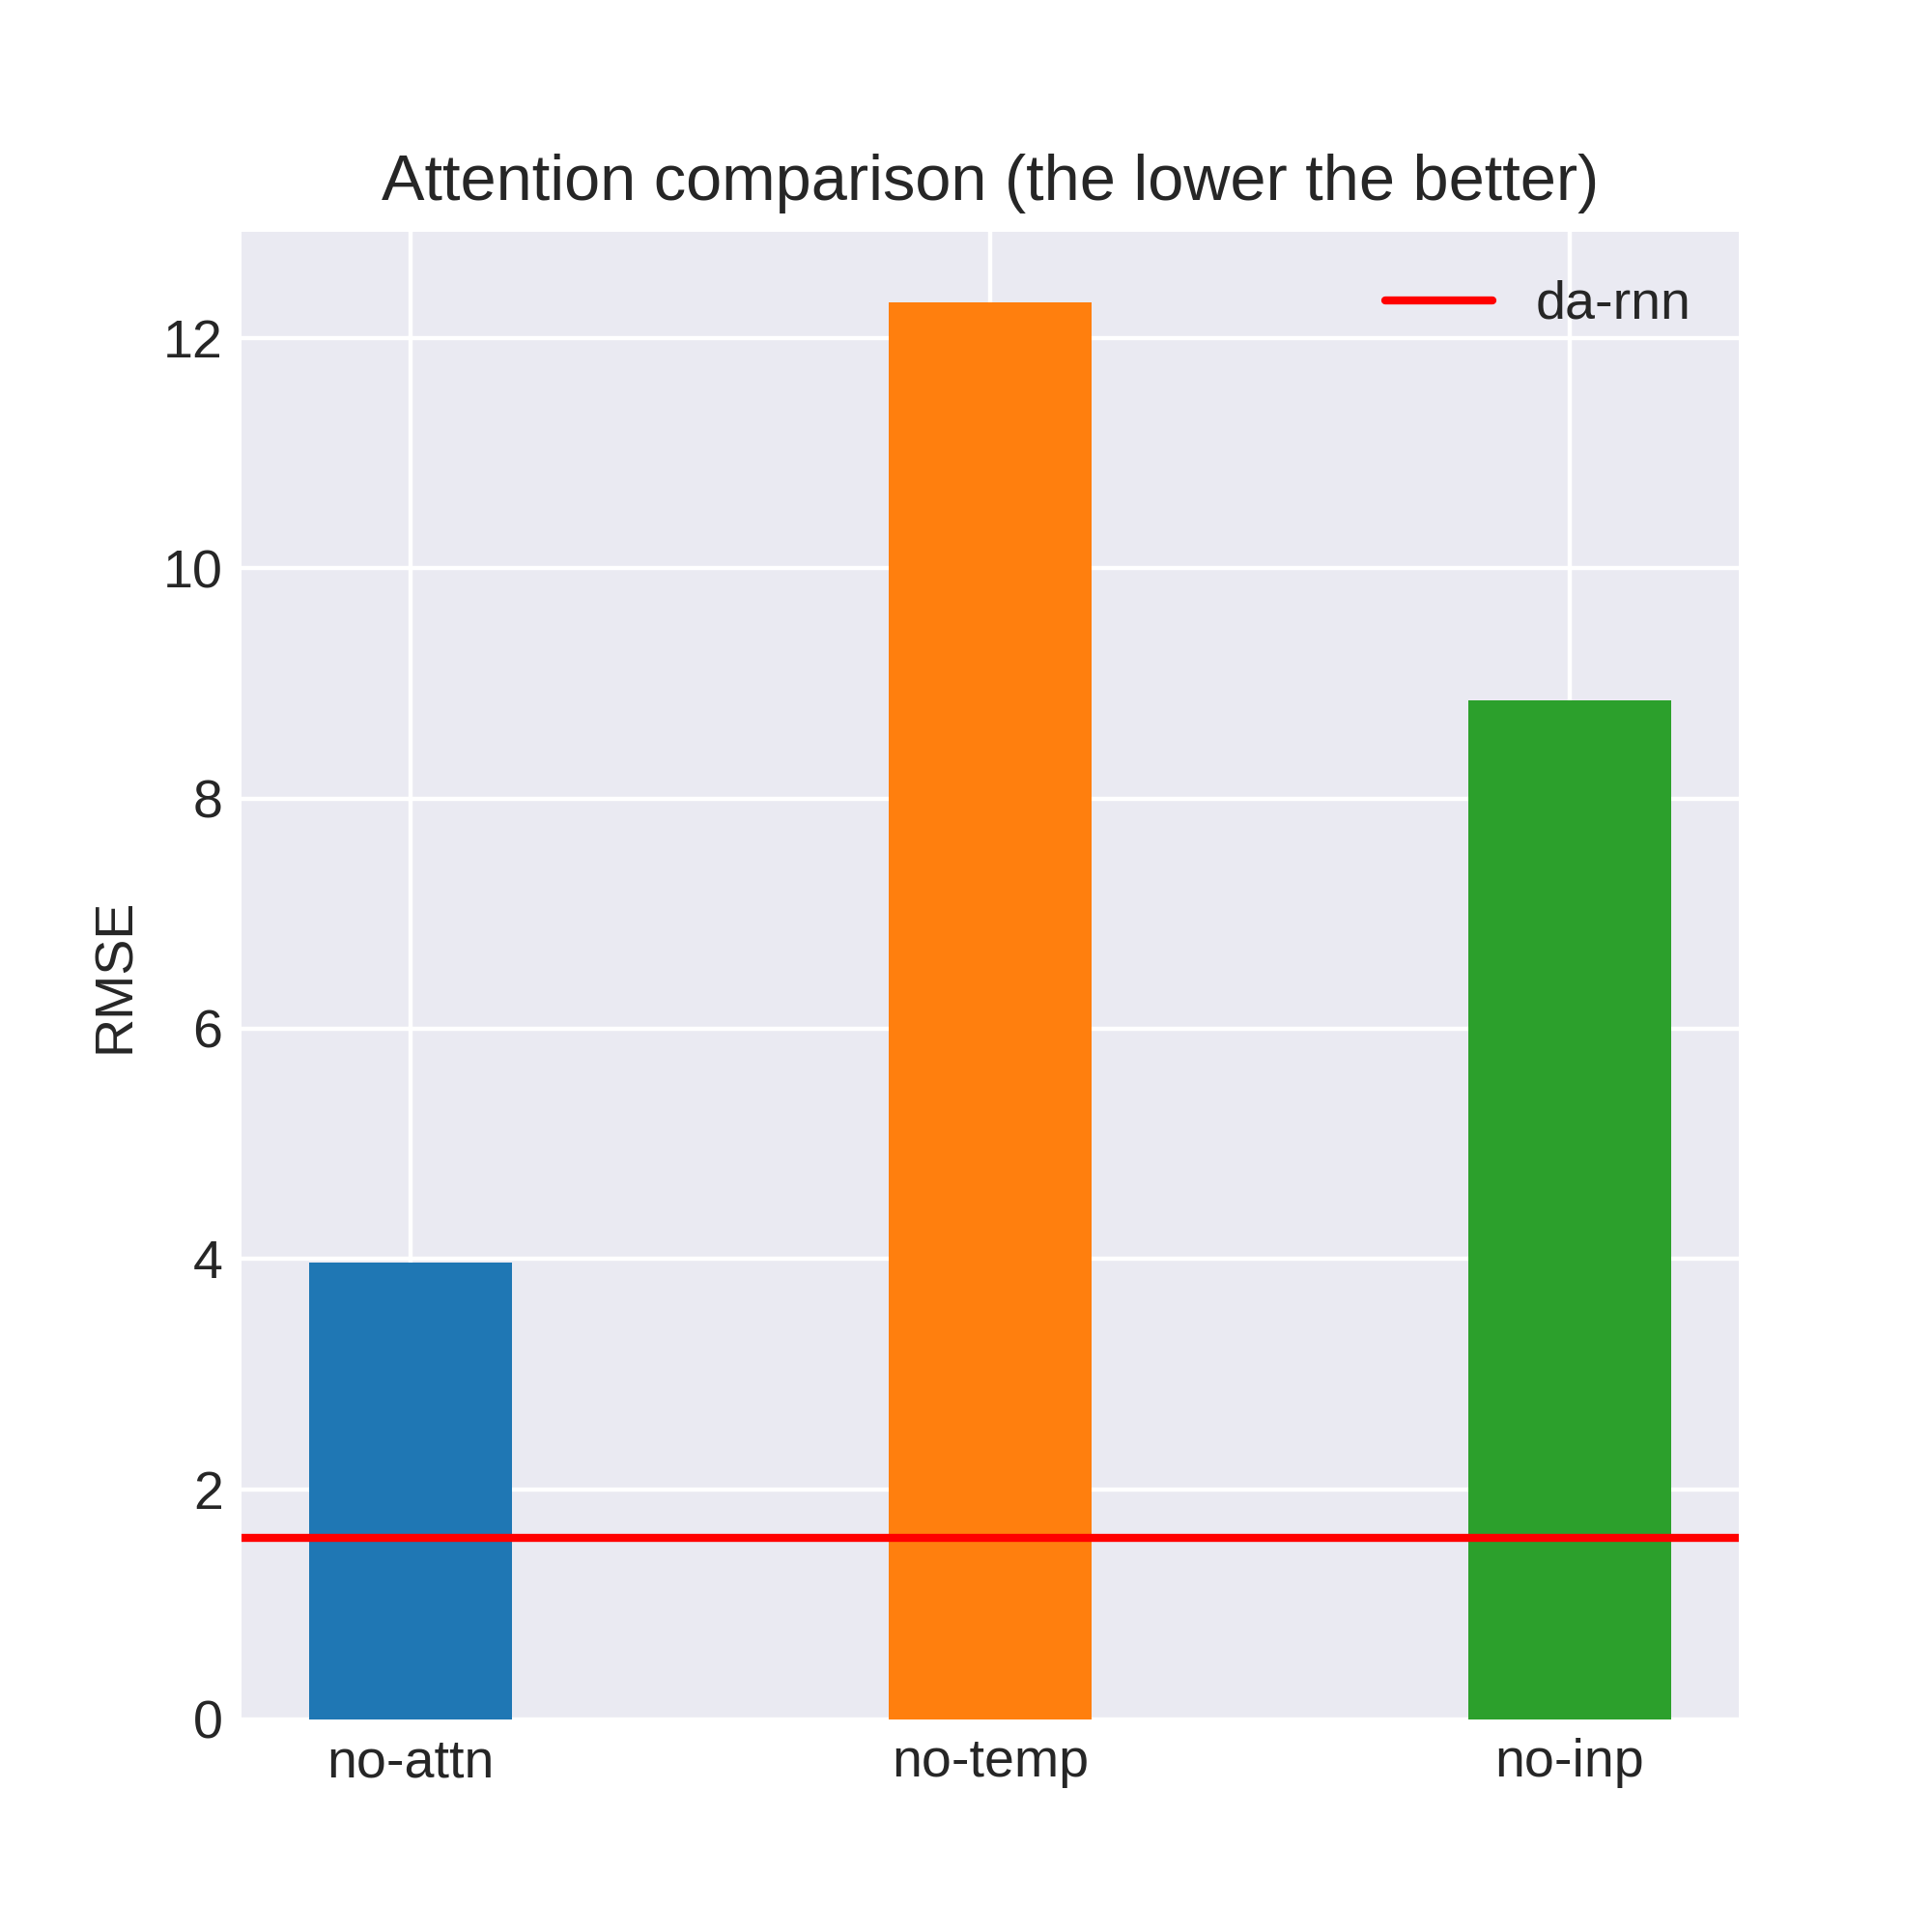
\includegraphics[width=0.4\linewidth]{ablation-nasdaq.png}
    \label{fig:ablation-nasdaq}
  }}
  \caption{Comparison of the performances by switching off the attention
  mechanisms. The red line shows the RMSE score of the model with both
  attentions (input and temporal attention) enabled. In blue the RMSE score
  with both the input and temporal attentions disabled. In orange the score
  with only the temporal attention disabled and in green the score with
  only the input attention disabled. Similar plots for the other metrics.}
  \label{fig:ablation}
\end{figure}

To validate the usefulness and correctness of the dual-stage attention approach
we perform an ablation study of the model and report the values of the
resulting three systems comparing them against the model with both attention
mechanisms active and hyperparameters said above. We notice that here we
include the temporal-attention-only model together with the
input-attention-only model that was not evaluated in our original reference
paper.

In Figure \ref{fig:ablation} the comparison between the model without any
attention mechanism, without the temporal attention and without the input
attention respectively is shown against the line representing the dual
attention model of the authors'.

Figure \ref{fig:ablation-sml} shows that the temporal attention is
ineffective for this task (green bar and red line representing
models with temporal attention enabled higher than models
where the temporal attention is disabled). This is probably due to the
sinusoidal shape of the target series of which timesteps have equal
importance.

Figure \ref{fig:ablation-nasdaq} highlights the effectiveness of the
dual-stage attention mechanism. In the NASDAQ100 dataset the models
without one of the attention mechanisms are not able to produce
remarkable results due to both the large number of driving series and
the strong variations of the series over the timesteps.

\section{Simple encoder network baseline}

\begin{figure}[ht]
\centering
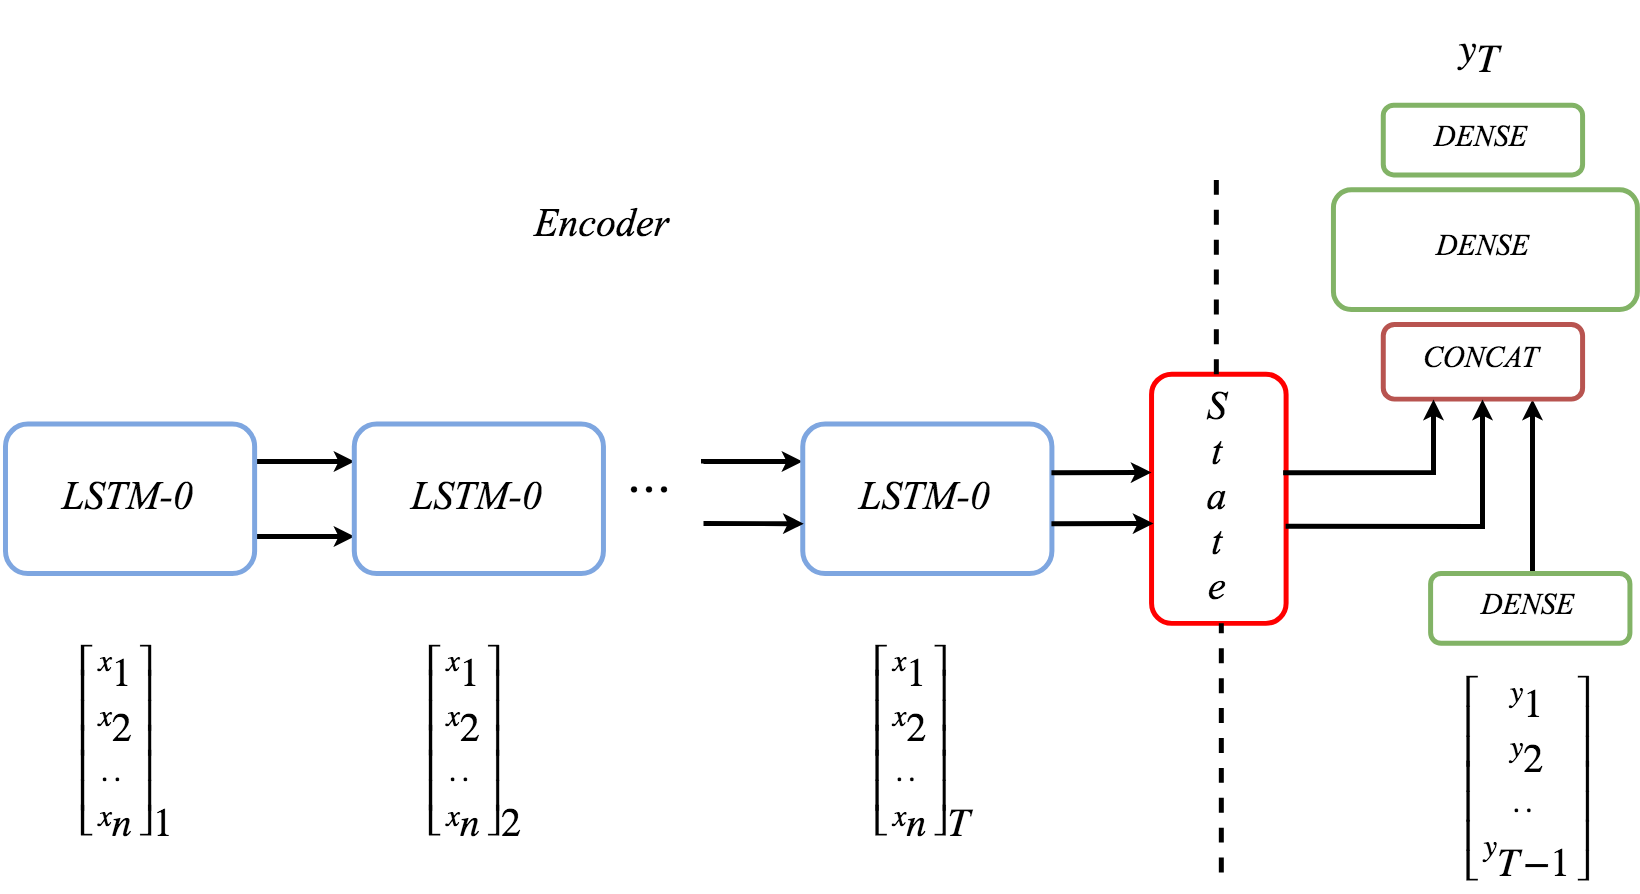
\includegraphics[width=0.9\linewidth]{ende-rnn-4.png} \\
\caption{Encoder model}
\label{fig:ende-rnn}
\end{figure}


In this paragraph we introduce a simple model we used as a baseline. 
We initially developed a model composed of an encoder and a decoder with the goal 
of producing a decoder network that could be easily extended to a multistep-ahead 
environment where we could predict accurately the future values for more than a 
single timestep.
So for the encoder of the original model we stacked two LSTM layers and collected 
the final output as the set of the two hidden states and cell states. These 
vectors represent the driving series. For the decoder part we set as initial 
state of the decoder LSTM the output of the encoder. 
We notice that the number of layers in the decoder had to be
the same as the encoder, as well as the dimension of the hidden sizes. 
We then give as input to the decoder LSTM the vector containing the past history 
of the target series and we feed this vector to the cell at each time-step. The 
output hidden state of the decoder is fed to a dense layer to obtain the final 
value for the desired timestep.

Discouraged by the difficulties this network had in learning to predict values 
for the NASDAQ 100 dataset (although the model still performed well on the 
SML2010 dataset) we decided to make the network simpler focusing only on the 
single step target series value forecasting. Given this choice we dropped 
completely the decoder part replacing it with two feed-forward neural networks 
one encoding the target series history, and one that takes the concatenation of 
encoder hidden and cell state of the final LSTM iteration with the output of the 
first dense layer and maps it to the predicted value of the target series.

For the encoder network we mostly left it unchanged, we 
just reduced the number of LSTM layers from 2 to 1; the choice of keeping the 
encoder makes sense since we still want to capture time dependencies in the 
driving series and encode this information in a fixed size representation. On the 
other hand the window of past values is considered altogether applying a dense 
layer to the input vector.


\subsection{Implementation details}

For this simple encoder model we took advantage of the Keras. We instantiate a
\texttt{LSTMCell} and gave it as argument to a \texttt{RNN} layer. Using the
functional API we applied this layer to the driving series' input and collected
the final state. As in the original architecture the input to the LSTM at each 
timestep is a vector if $n$ values of the $n$ driving series for that timestep.

Finally we apply a \texttt{Dense} layer to the concatenation of the encoder 
hidden and cell states and to the values of the past history for the target 
series. The concatenation of the results is passed to two final \texttt{Dense} 
layers up to the output with the predicted value.

We finally defined a callback in the \texttt{fit()} function call to make the
training stop if the value of the loss doesn't improve for a certain number of
consecutive steps (the level of patience was empirically adjusted).

We trained for a total of 100 epochs with an Adam optimizer without any learning 
rate decay.

\subsection{Results}

As you can see from the table of the values we got for the various metrics the 
model doesn't perform as well as the dual-stage attention RNN described in the 
previous sections. This validates the ideas by the original authors and finally 
justifies the complexity of the network with an improvement in the 
performance.


\begin{center}
\begin{table}
\begin{tabular}{r|c|c|c|c|c|c|c|c|c|}
\multicolumn{1}{r}{}
  & \multicolumn{3}{c}{\textbf{Train}}
  & \multicolumn{3}{c}{\textbf{Validation}}
  & \multicolumn{3}{c}{\textbf{Test}} \\
  \cline{2-10}
  & \multicolumn{1}{c}{RMSE}
  & \multicolumn{1}{c}{MAE}
  & \multicolumn{1}{c|}{MAPE}
  & \multicolumn{1}{c}{RMSE}
  & \multicolumn{1}{c}{MAE}
  & \multicolumn{1}{c|}{MAPE}
  & \multicolumn{1}{c}{RMSE}
  & \multicolumn{1}{c}{MAE}
  & \multicolumn{1}{c|}{MAPE}\\
\cline{2-10}
NASDAQ100 & 4.5726 & 3.5723 & 0.0744 & 4.0200 & 3.1977 & 0.0658 & 4.0803 &
3.1980 & 0.0647 \\
\cline{2-10}
SML2010 & 0.1049 & 0.0746 & 0.3858 & 0.1714 & 0.1714 & 0.5728 & 0.1026 & 0.0750
& 0.3497 \\
\cline{2-10}
\end{tabular}
\vspace{1em}
\caption{Results over SML2010 and NASDAQ100}
\label{results-encoder}
\end{table}
\end{center}

\section{Conclusion}

TODO

\newpage
\section*{References}
[1] Qin, Yao, et al. “A Dual-Stage Attention-Based Recurrent Neural Network for
Time Series Prediction.” Proceedings of the Twenty-Sixth International Joint
Conference on Artificial Intelligence, 2017.

[2] Cho, Kyunghyun, et al. “On the Properties of Neural Machine Translation:
Encoder–Decoder Approaches.” Proceedings of SSST-8, Eighth Workshop on Syntax,
Semantics and Structure in Statistical Translation, 2014.

\end{document}
